

\noindent 
\textbf{\stepcounter{zadatak}
\thecjelina.\thezadatak.}
%\begin{wrapfigure}{r}{0.3\textwidth} %this figure will be at the right
%    \centering
%    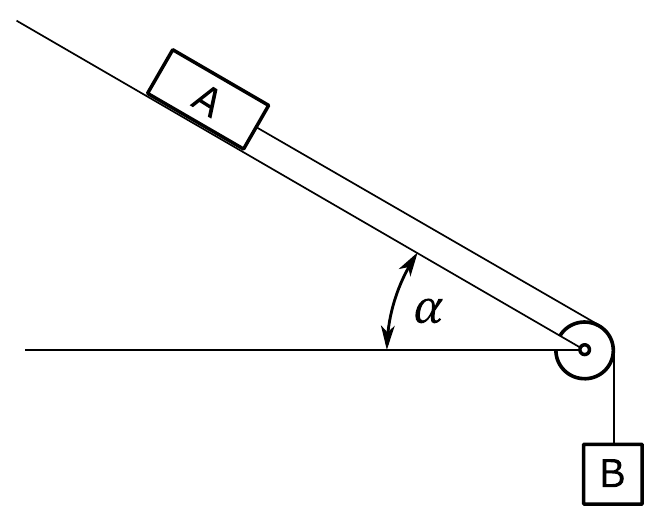
\includegraphics[width=0.3\textwidth]{03_Dinamika_materijalne_tocke/kosina_5_2.png}
%\end{wrapfigure}
Na slici  je sustav od dva utega mase $m_A=10\ kg$ i $m_B=5\ kg$. Uteg B povezan je tankom nerastezljivom niti s utegom A. 
Kosina na kojoj se nalazi uteg A nagnuta je pod kutom $\alpha=30^\circ$, a koeficijent kinetičkog trenja između kosine i utega A iznosi $\mu_k=0,2$.
\begin{enumerate}[label=\alph*)]
 \item Skicirajte problem i označite sve sile i smjer gibanja (vektor ubrzanja) cijelog sustava.
 \item Izračunajte iznos ubrzanja cijelog sustava.
 \item Izračunajte iznos sile napetosti niti.
\end{enumerate}

\begin{figure}[ht]%{r}{0.7\textwidth} % Inline image example
  \begin{center}
    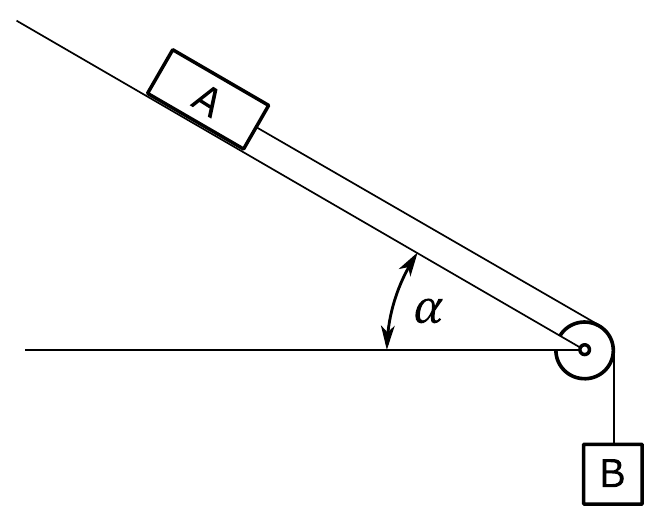
\includegraphics[scale=0.25]{../03_Dinamika_materijalne_tocke/Zadatak_D701.png}
  \end{center}
  %\caption{Fish}
\end{figure}
